\documentclass{standalone}
\usepackage{tikz}
\begin{document}
\scalebox{0.5}{%
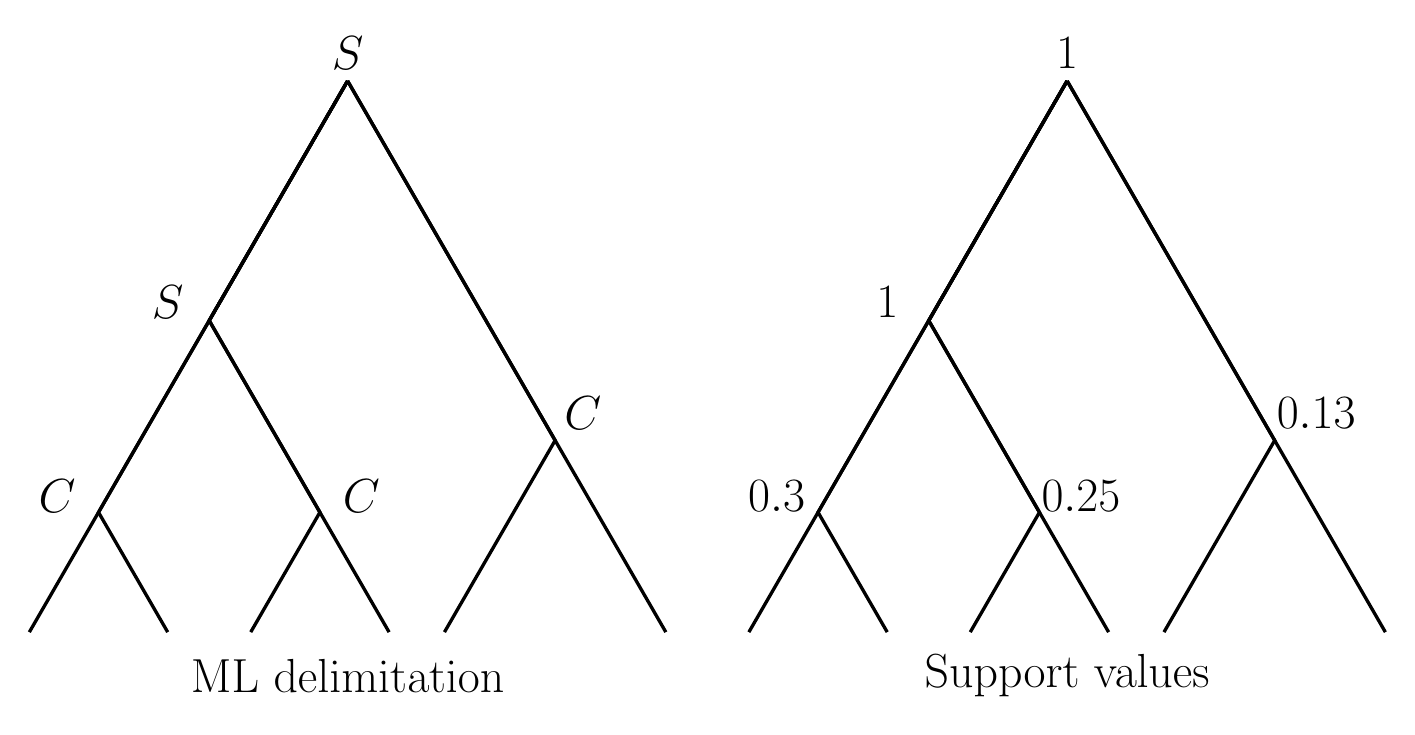
\begin{tikzpicture}[font=\tiny]
%
% define constants 
%
%\newcommand*{\WIDTH}{55}
%\newcommand*{\HEIGHT}{25}
%%
%% create a grid for easier drawing
%%
%\draw[step=1em,gray,very thin] (0,0) grid (\WIDTH em,\HEIGHT em);
%%
%% draw x axis
%%
%\foreach \i in {0,...,\WIDTH}
%{
%  \node at (\i em, -1 em) {\i};
%}
%%
%% draw y axis
%%
%\foreach \i in {0,...,\HEIGHT}
%{
%  \node at (-1 em,\i em) {\i};
%}

% draw ML delimitation

\newcommand*{\Offset}{260}%

\draw[very thick] (12.5 em, 22em) -- ++(240:23em);
\draw[very thick] (12.5 em, 22em) -- ++(300:23em);


\draw[very thick] (12.5 em, 22em) -- ++(240:18em) -- ++(300:5em);
\draw[very thick] (12.5 em, 22em) -- ++(240:10em) -- ++(300:13em);
\draw[very thick] (12.5 em, 22em) -- ++(240:10em) -- ++(300:8em) -- ++(240:5em);

\draw[very thick] (12.5 em, 22em) -- ++(300:15em) -- ++(240:8em);

\node[font=\LARGE] at (12.5em, 23em) {$S$};
\node[font=\LARGE] at (6em, 14em) {$S$};
\node[font=\LARGE] at (2em, 7em) {$C$};
\node[font=\LARGE] at (13em, 7em) {$C$};
\node[font=\LARGE] at (21em, 10em) {$C$};

% draw delimitation with support values

\draw[very thick] (\Offset+12.5 em, 22em) -- ++(240:23em);
\draw[very thick] (\Offset+12.5 em, 22em) -- ++(300:23em);


\draw[very thick] (\Offset+12.5 em, 22em) -- ++(240:18em) -- ++(300:5em);
\draw[very thick] (\Offset+12.5 em, 22em) -- ++(240:10em) -- ++(300:13em);
\draw[very thick] (\Offset+12.5 em, 22em) -- ++(240:10em) -- ++(300:8em) -- ++(240:5em);

\draw[very thick] (\Offset+12.5 em, 22em) -- ++(300:15em) -- ++(240:8em);

\node[font=\LARGE] at (\Offset+12.5em, 23em) {$1$};
\node[font=\LARGE] at (\Offset+6em, 14em) {$1$};
\node[font=\LARGE] at (\Offset+2em, 7em) {$0.3$};
\node[font=\LARGE] at (\Offset+13em, 7em) {$0.25$};
\node[font=\LARGE] at (\Offset+21.5em, 10em) {$0.13$};


\node[font=\LARGE] at (12.5em, 0.5em) {ML delimitation};
\node[font=\LARGE] at (38.5em, 0.5em) {Support values};

\end{tikzpicture}}
\end{document}
